\section{Audio Preprocessing}


Audio preprocessing is an essential step that is performed on audio data before it is fed into machine learning models. The objective of audio preprocessing is to clean the collected audio data, extract relevant features, and transform the data into a format that can be easily interpreted by the models. This section discusses important aspects of audio preprocessing, including noise reduction and audio trimming, and how we employed them.

\subsection{Noise Reduction}

One of the key techniques used in audio preprocessing is noise reduction. In audio data, noise can arise from a variety of sources, such as background noise, microphone interference, or electrical interference. The presence of noise in the audio data can significantly impact the performance of any audio classification system.

One common strategy for denoising audio is spectral gating, which involves gating the signal only on high-level sounds. We recurred to the \textit{noisereduce} library to implement this noise reduction technique.
This algorithm estimates a noise threshold for each frequency band of the signal. This threshold is used to compute a mask, which gates noise below the frequency-varying threshold. The code snippet \ref{nr:code} shows how we implemented the noise reduction technique.

\begin{listing}[H]
	\begin{minted}{python}
noisereduce.reduce_noise(
	y=y, sr=16000, n_fft=2048, hop_length=512, prop_decrease=.75, time_constant_s=1
)
	\end{minted}
	\caption{Python code for applying noise reduction using the \textit{noisereduce} library.}
	\label{nr:code}
\end{listing}


\subsection{Audio Trim}

Another important aspect of audio preprocessing is audio trimming. This technique involves removing unwanted portions of the audio signal that are not relevant. Trimming the silence from the beginning and end of an audio clip is a common technique in speech-based classifications. This reduces the computational overhead and also makes the data more manageable.

We defined 30 decibels as the threshold for considering silence and removed any segments, at the beginning and end of the audio, that fell below this threshold. This was done because 30 decibels is generally considered a very low level of noise, and is often used as a standard threshold for measuring background noise levels in quiet environments.

Table \ref{trim_durations} shows the original and after trim durations for all of the \ac{iemo} audio files, and it is clear that this process of removing unwanted noise at the beginning and end of the audio files resulted in overall shorter audio durations.

\begin{table}[H]
	\centering
	\caption{Audio files' original and after trim durations.}
	\label{trim_durations}
	\begin{tabular}{lrr}
		\toprule
		Metric & Original Duration & After Trim Duration \\
		\midrule
		Minimum  		&  0.585 	&  0.256 \\
		25th Percentile &  2.324	&  1.952 \\
		%50th Percentile	&  3.577	&  3.109 \\
		Mean 			&  4.549  	&  4.065 \\
		75th Percentile	&  5.773	&  5.248 \\
		Maximum 		& 34.139   	& 33.184 \\
		\bottomrule
	\end{tabular}
\end{table}



\subsection{Conclusion}

Figure \ref{fig:prep} compares an original and preprocessed audio file from the \ac{iemo} dataset. We observed the amplitudes of the preprocessed waveform are reduced and that there are more silent parts compared to the original. The preprocessed spectrogram shows a cleaner representation and some reduction of decibels values. The preprocessed power spectral density also contains lower values of dB/Hz, and, for example, in frequencies around 1100 and 1900 Hz, the elimination of some spike values can be perceived. In addition to these observations, we also listen to the resulting audio and manually detected noise reduction and a clearer sound.

\begin{figure}[H]
	\centering
	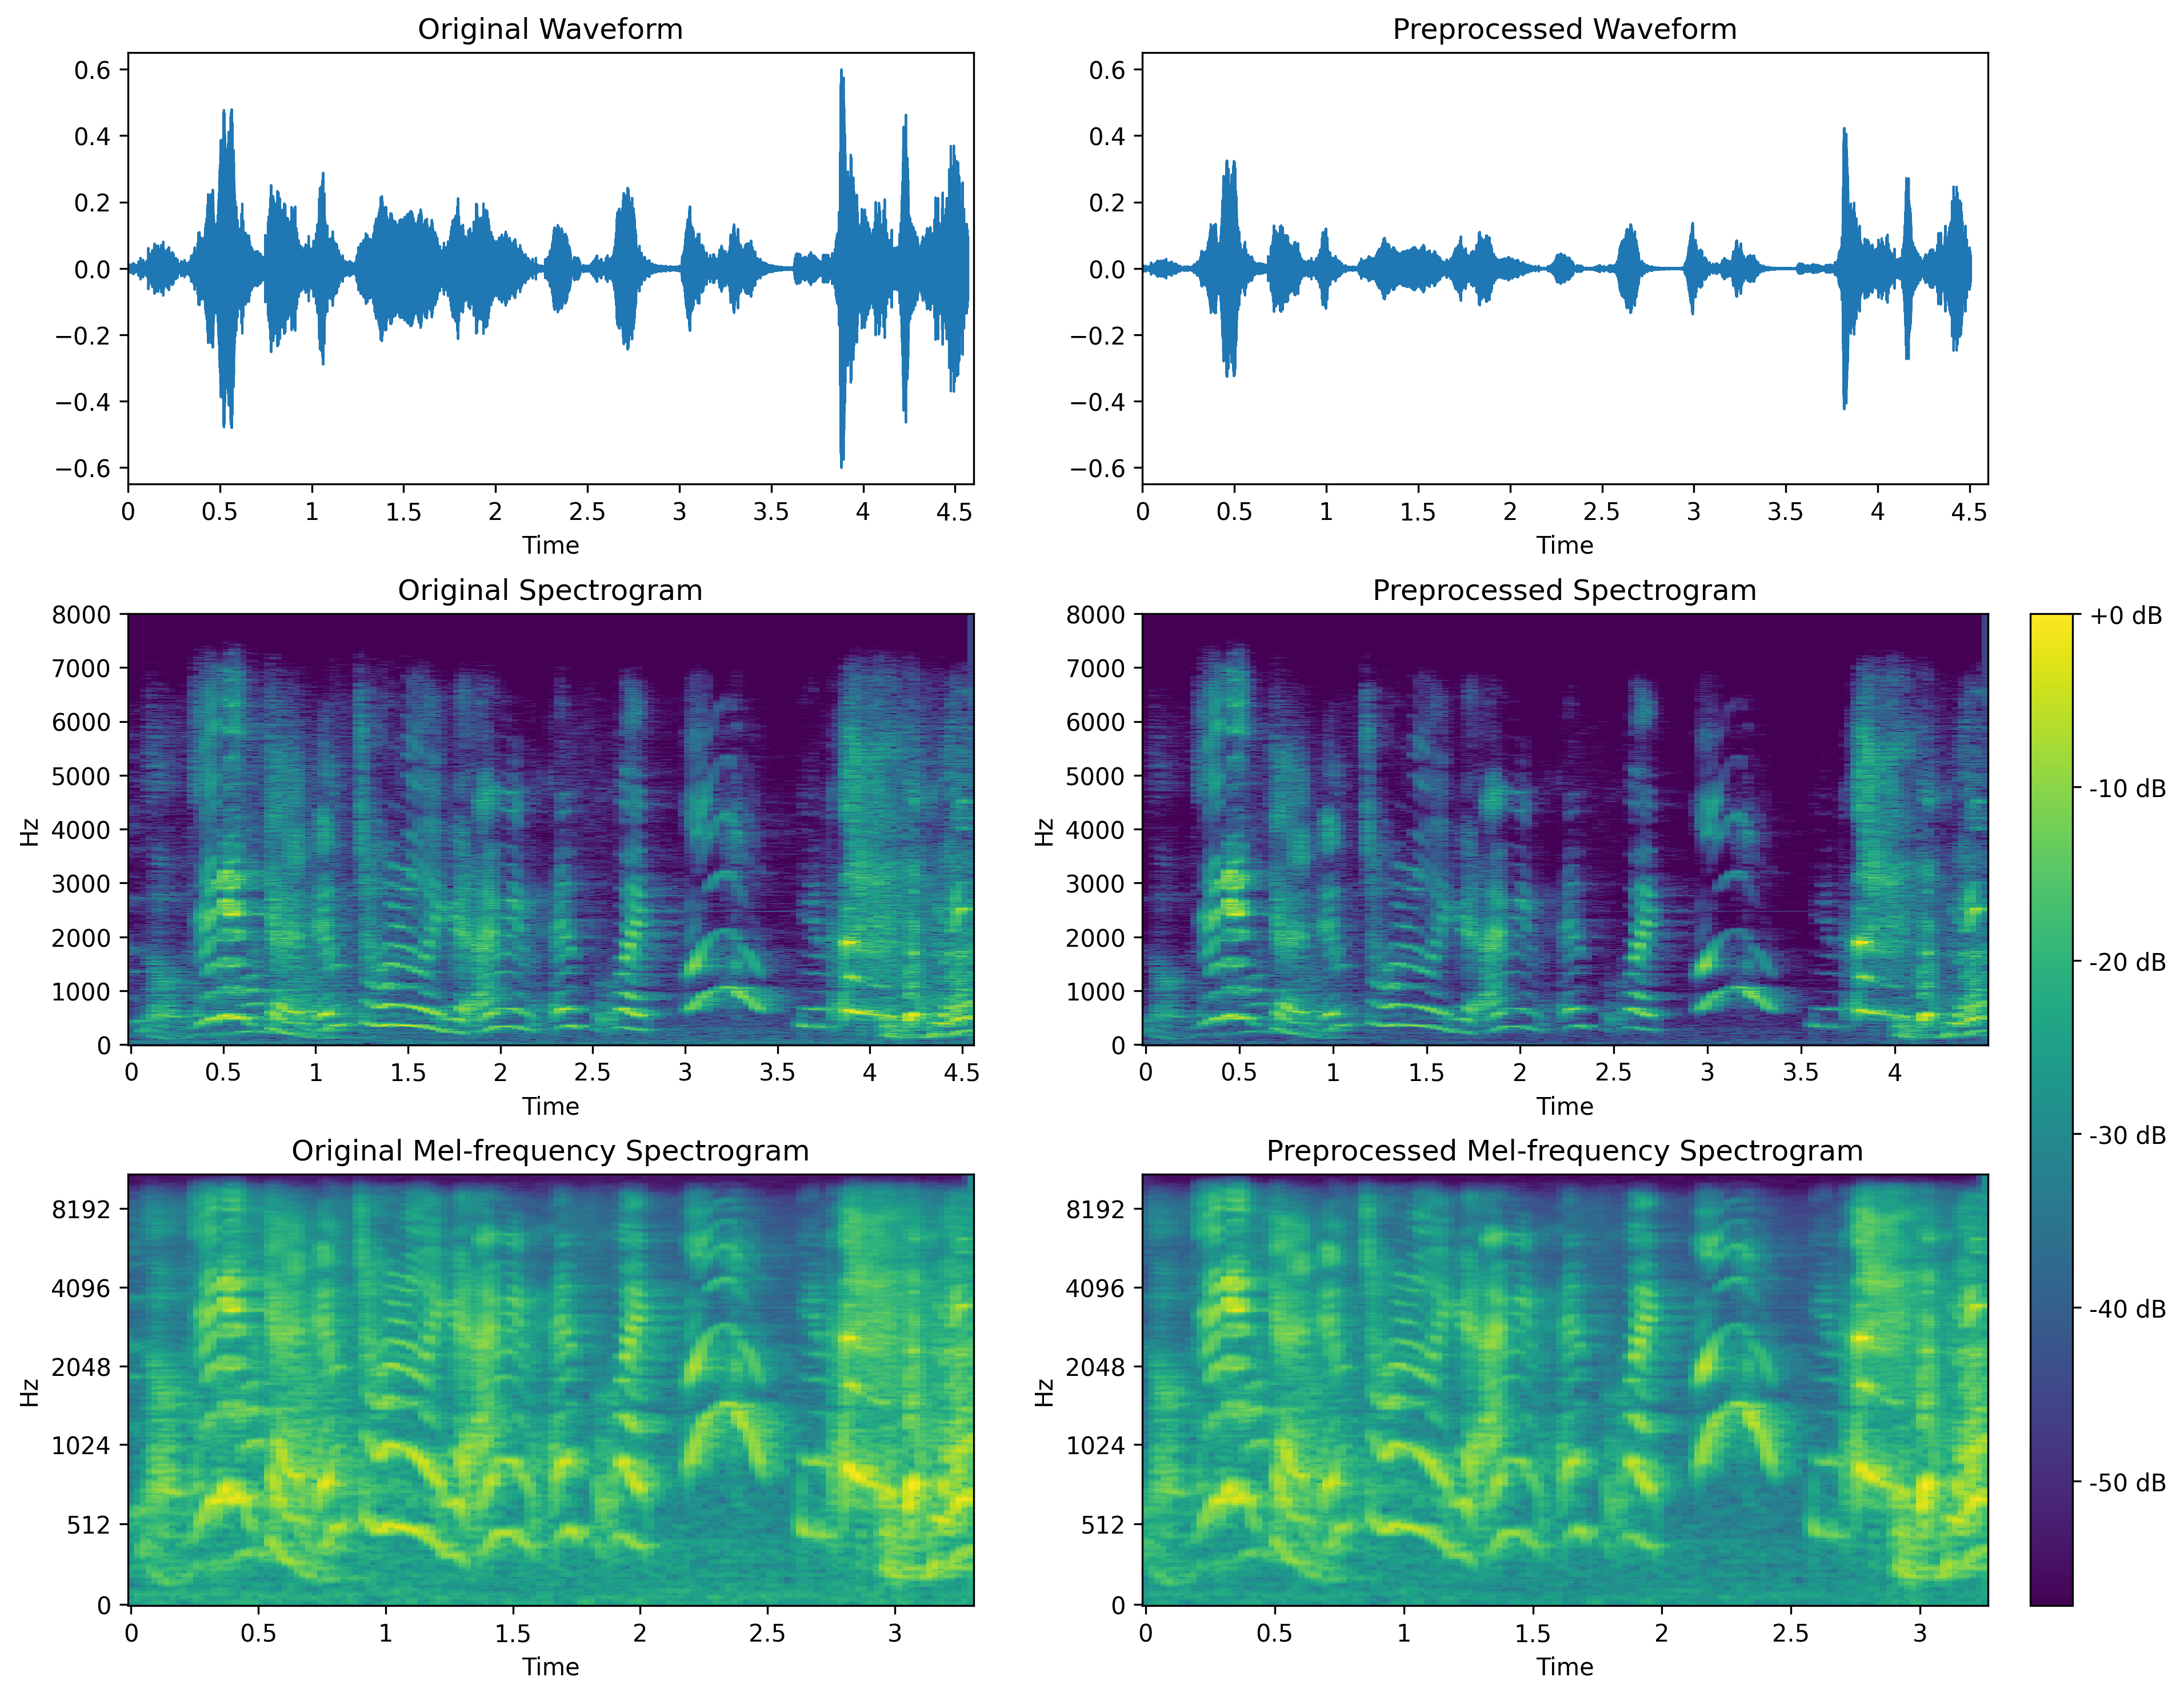
\includegraphics[width=\textwidth]{figs/4_2_preprocessing/preprocessing.png}
	\caption{Visual representations of audio features before and after preprocessing.}
	\label{fig:prep}
\end{figure}

These results demonstrate that the employed techniques cleaned the audio data, resulting in shorter durations and less noise. Overall, this audio preprocessing is an essential step to ensure the quality of any type of audio classification, but it requires an in-depth comprehension of audio signals to create a successful preprocessing pipeline since it can cause a great drawback in some scenarios where noise may be part of the signal of interest, and removing it may lead to misinterpretation.
